
\section{Individual Path finding}\label{sec:ipf}
This section describes functions that can be used as cost/objective function. This means it can be maximized, minimized in order to obtain paths with different properties.

\subsection{Formalization}

Individual Path Finding (IPF) aims to compute for each agent, a non-empty set of paths. IPF can be summarized as ``MAPF without collisions''; it takes the same input as MAPF (see \ref{sec:background}), it however differ on the output. The output is a triple \((V,E,\tau)\) where \(\tau\) is a set where the relation is bijective, considering an agent \(a \in A\), we have  \(\tau[a]\) being a non-empty set of path, we can refer to \(\tau[a]\) with \(\gamma\) or \(\gamma_a\) if necessary for better understanding or lighter notation. Let an agent \(a=(s,g)\), for any \(\pi\in \gamma_a\), \(\pi(0) = s\) and \(\pi(|\pi|-1) = g\). Thus, every paths composing \(\gamma\) can have a different length.


We will then list and classify what can be the different kind of paths that can compose \(\tau\), what are their properties, advantages and inconvenient.


We also define the \(pick\) function which allows lighter notation; \(pick\) takes as input a set of paths \(\gamma\) and returns one of the paths in \(\gamma\).




\subsection{Properties of a Path}

\subsubsection{Path of defined length}
A noticeable property is the \textbf{length} of the path, denoted as \(|\pi|\). We can distinguish two cases; the length is the minimal possible or it is strictly higher than the minimal. The first case gives us a lower bound for searching a solution, and if a solution exists using only shortest path, it is an optimal solution. In the second case optimality is no longer guarantee. However, working with path of defined length, combined with knowledge of the graph, it can make the ``field of action'' for the merging algorithm wider, which can result of finding a solution, but also rise the number of possibilities which can lead to more computing difficulties.


\begin{definition}[Shortest Path (SP)]\label{def:shortest_path}
  Given an initial and a final position, an associated path \(\pi\) is in the set \(SP\) if \(\pi\) is valid and no path \(\pi'\) such as \(|\pi| > |\pi'|\). Generally, \(SP\) the set of all of the shortest path possible for a given initial and final position. For lighter notation, \(|SP^i|\) to the size of  paths \(\pi\) composing \(SP\)
\end{definition}



\(2k\) paths are specific paths of defined length, they are of length \(|SP| + 2k\) where \(k\) is a positive integer. The \(2k\) section represents the fact that in order to ``resolve'' a conflict, if wait moves are not possible for any reason (specification, approaches, instance\ldots), solving a conflict would require at least two moves. This kind of paths comes with an assumption; computing an additional path of \(2k\) kind is (way) faster than trying to solve a conflict in the solver. Intuitively, this kind of paths can be quite interesting to solve~\nameref{def:blocking_agent} instances.





\subsubsection{Path containing bending(s)}

Counting bending in a path require to work on a graph using cartesian coordinate system. From coordinates we can compare angles of the vectors made from the current vertex and the previous one, to the current one and the next one. If angles are equals, it means that the path is continuing in its previous direction (angles have the same direction), otherwise a direction change is identified. Formally, we can define a bending in an cartesian coordinate system of the path \(\pi\) at time step \(t\) as such: \[
 u = \overrightarrow{(\pi(t-1),\pi(t))} \text{ and  } v = \overrightarrow{(\pi(t),\pi(t+1))}
\]
\[
  bending(\pi,t) = 
    \begin{cases}
      1  & \text{if }  \widehat{u} = \widehat{v} \\
      0  & \text{otherwise}
    \end{cases}  
\] Then, the number of bending in a path is \[
  Bending(\pi) =  \sum_{t=1}^{|\pi|-2}{bending(\pi,t)}
\] 

If a ``waiting'' move is considered as a vector of size 0, by definition, any vector of size 0 is ``perpendicular'' to any other one.

It is important to mention that approach for counting bendings makes sense for a grid scenario with defined and restricted directions; there high chance that bendings definition should be changed for scenarios working with continuous directions or a 3+ dimension. 
Given the number of bending, we can deduce information; with zero bending, we can trivially deduce that the initial position and the goal position are on the same column or row, furthermore the path is in \(SP\).




\subsection{Path using information coming from the graph}
In this section, we will describe what information we can deduce from a path in the graph individually. 
\subsubsection{Degree of the path}
The degree of the path is calculated by using the in and out degree of vertices (which is the number of edges linked to the vertex) that the path is going through; formally, we have for \(v\in V\) and \[
  degree^+(v) = \sum^{\forall v\in V}{ 
    \begin{cases}
    1 & \text{if } \exists (v,v') \in E \\
    0 & \text{otherwise}  
    \end{cases}}
\] 
\[
  degree^-(v) = \sum^{\forall v'\in V}{  
    \begin{cases}
    1 & \text{if } \exists (v',v) \in E \\
    0 & \text{otherwise}  
    \end{cases}}
\] 

% n(e) = v, where e = (v,u)
% in_edges(v) = { e | in(e) = v} 
% degree(v) = |in_edges(v)| 


We can then calculate the degree of a path; \[
  Degree(\pi) = \sum_{t=1}^{|\pi|-1} degree^+(\pi(t)) + degree^-(\pi(t))
  \] Knowing this information, we can tell if a path is ``going next to wall'' or more ``going through the middle'' of the environment. We can of course imagine using only in or out degree information. \(Degree\) works for a directed graph, notion of in out degree get lost for a non-directed graph, however we can easily change \(degree^+\) and \(degree^-\) by  \[
    degree(v) = \sum^{\forall e\in E}{ 
      \begin{cases}
      1 & \text{if } v\in e \\
      0 & \text{otherwise}  
      \end{cases}}
  \]

Figure \ref{img:criteria_degree} shows an example of two paths for a single agent. The red path is obtained by selecting nodes that have the highest degree while the green path is obtained by choosing nodes that have the lowest degree.   
\begin{figure}[H]
  \centering
  \caption{Example of paths based on the degree of vertices}\label{img:criteria_degree}
  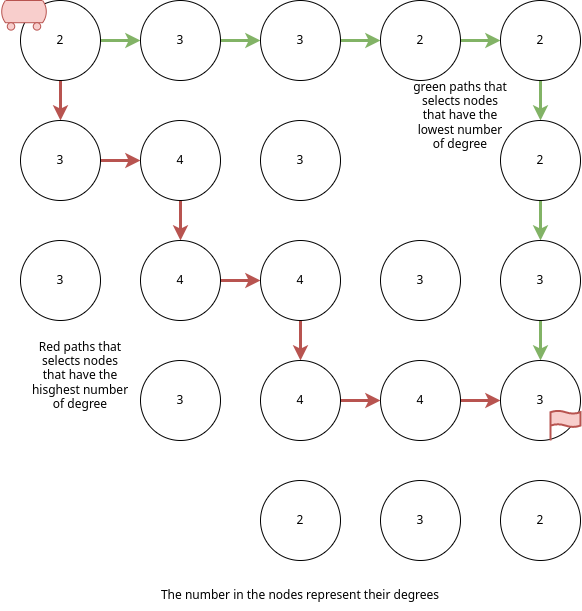
\includegraphics[width=\widthimg]{img/criteria_degree.drawio.png}
\end{figure}


\subsubsection{Coverage of the graph}\label{sec:graph_coverage}

Coverage of a graph represents the proportion of the graph that is used by an agent. We can define graph coverage as such: \[
  coverage(\pi) = \frac{|vertex(\pi)|}{|V|}
\] Graph coverage definition changes given the input; \[
  coverage(\gamma) = \frac{| \bigcup^{\pi \in \gamma} vertex(\pi) |} {|V|}
\] Finally, \[
  coverage(\tau) = \frac{| \mathlarger{\mathlarger{\bigcup}}^{\gamma \in \tau}{ \text{  } \bigcup^{\pi \in \gamma}{vertex(\pi)}} |} {|V|}
\] where \(vertex(\pi)\) is a function that returns the associated vertices set of the sequence of vertices.


\subsection{Selection of one path considering other agents}

\subsubsection{Path conflict}
Potential conflict represents a function counting conflict occurring between agents considering time step. It takes as input a set of path \(\tau\); formally we define first \[
    pc(\pi,\pi') =   \sum_{t}^{min(|\pi|,|\pi'|)}{
        \begin{cases}
            1   & \text{if  } conflict(\pi,\pi',t) \\
            0   & \text{otherwise}
        \end{cases}
    }
\] Where \(conflict\) returns the boolean value ``true'' if any conflict occurs between \(\pi\) and \(\pi'\) at time step \(t\), return ``false'' otherwise. Furthermore, \(pc\) does not forbid \(\pi\) and \(\pi'\) belonging to a same \(\gamma\).

We can then compare sets of paths:
\[ 
  pathc(\gamma,\gamma') = \mathlarger{\sum}_{\pi,\pi'}^{\forall \pi \in \gamma,\forall \pi' \in \gamma'}{
        pc(\pi,\pi')
    }
\] where \(\gamma\) an \(\gamma'\) are different sets of path, typically coming from \(\tau[a_{\in A}]\) and \(\tau[a'_{\in A}]\). We can then define \[
    PathC(\tau)= \sum_{a,a'}^{\forall a \neq a' \in A}{
        pathc(\tau[a],\tau[a'])
    }
\]

Another interesting function would be to compare a single path to a set of path \(\gamma\) or \(\tau\), indeed comparing all of the set of agents to all others, if their respective set of paths are large, the meaning of the comparison becomes blurry. We can in consequences define other functions that aims to keep interesting result not matter how much paths it takes as input:

\[ 
  pathc(\gamma,\pi) = \mathlarger{\sum}_{\pi'}^{\forall \pi' \in \gamma}{
        pc(\pi',\pi)
    }
\] and \[ 
    pathc(\tau,\pi) = \mathlarger{\sum}_{\gamma}^{\forall \gamma \in \tau}{
        pathc(\gamma,\pi)
    }
\]

Another point to mention is that the definition is not complete; if two paths have different length, a part of the bigger path will not be considered

\subsubsection{Blocking agent}\label{def:blocking_agent}
  An agent \(a\) is called a ``blocking agent'' towards \(a'\), or agent \(a\) is blocking agent \(a'\), if at time step \(t\), all the next vertices from \(\pi_a(t)\) to \(\pi_a(|\pi_a|-1)\) are included in the vertices from \(\pi_{a'}(t)\) to \(\pi_{a'}(|\pi_{a'}|-1)\), for instance see figure\ref{img:blocking_agent} where red agent, at time step 1, is blocking the blue agent. Formally we have: \
  \[
    blocking(\pi,\pi',t) = \begin{cases}
      true   & \text{if }  since(\pi,t) \subset  since(\pi',t) \\
      false  & \text{otherwise}
    \end{cases}
  \] (We read ``path \(\pi\) is blocking path \(\pi'\) at time step \(t\)"). Where the function \(since\) is define as:
  \[
    since(\pi,t) = \bigcup_{i=t}^{i \rightarrow |\pi|-1} \{\pi(i)\}  
  \] which represent the set of vertices in \(\pi\) from \(t\) until the end of the path .
  
  It is called  ``fully-blocking''  if  \(a\) is a blocking \(a'\) at time step 0 (also see figure\ref{img:blocking_agent}). 
\begin{figure}[H]
  \centering
  \caption{Example of blocking agent}\label{img:blocking_agent}
  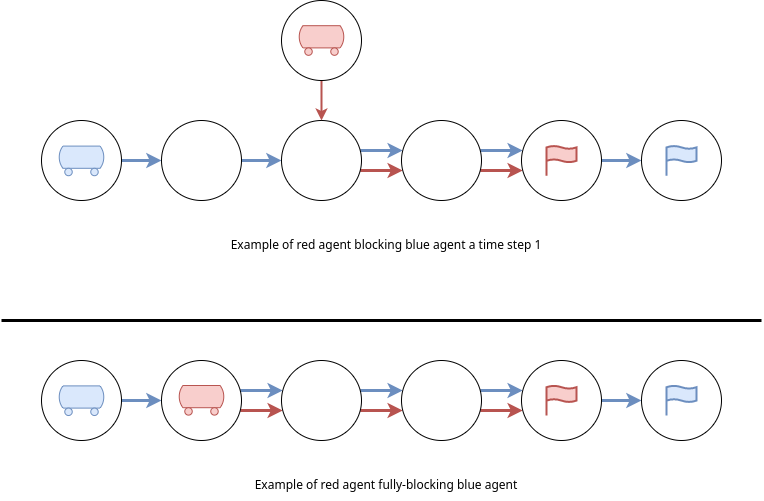
\includegraphics[width=\widthimg]{img/blocking_agent.drawio.png}
\end{figure}



\subsubsection{Potential conflict}
Potential conflict aims to count conflict occurring between paths without considering time step, in other words it delineate the union of common vertices between a all paths. it differs with path conflict by the fact that path conflict are defined according to time step, which is not the case for potential conflict. By definition, path conflict are specific cases of potential conflict, you can see as instance the figure~\ref{img:potential_conflict} which represent an isntance where no collision would occur, however there is a potential conflict represented by the yellow node. 

\begin{figure}[H]
  \centering
  \caption{Potential conflict}\label{img:potential_conflict}
  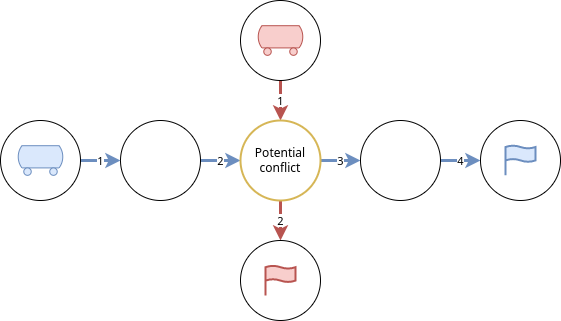
\includegraphics[width=\widthimg]{img/potential_conflict.drawio.png}
\end{figure} 

Formally, in order to define potential conflict, we have to define intermediate functions: \[
  potc(\pi,\pi') = |vertex(\pi) \cap vertex(\pi')|
\]
\[
  potentialc(\gamma,\gamma') = \mathlarger{\sum}_{\pi \in \gamma,\pi' \in \gamma'}{
    potc(\pi,\pi')
}
\]
\[
    PotentialC(\tau)= \sum_{a,a'}^{\forall a \neq a' \in A}{
        potentialc(\tau[a],\tau[a'])
    }
\]


We do not separate vertex conflict and edge conflict since it is by definition, included in the calculus; considering an edge conflict occurring a time step \(t\) (and \(t+1\)) between paths \(\pi\) and \(\pi'\), by definition, it means that \(\pi(t) =\pi'(t+1)\) and \(\pi(t+1) =\pi'(t)\). Thus, \(potc\) functions will count an edge conflict as two potential conflict. However, it could be interesting to separate potential edge conflict from potential vertices conflict.




% \subsubsection{Overused vertices}

% Overused vertices are vertices that are present in more than 

% \[
%   visited1^+(\tau) = \mathlarger{\mathlarger{\bigcup}}^{\forall a \neq a' \in A} (\forall\pi \in \tau[a] \cap \forall \pi' \in \tau[a']) 
% \]

\subsubsection{Conflict window}\label{sec:conflict_window}
A conflict window is defined with a couple of vertices \((v,v')\in V\) in a graph with orthonormal coordinate system, we also introduce the function \(coordinate:  V \rightarrow (\mathbb{N},\mathbb{N})\) which gives the coordinate associated to a vertex. Let \(C\) be a set containing all conflicts (these can be path or plan conflict), formally it can be define as \[
    C = \{v  | v \in V, conflict(v)\}
\] where \(conflict\) is a boolean condition; true if a conflict exist at vertex \(v\), else false. The next step is to ``draw" a rectangle (see \nameref{img:conflict_window} figure). To do so,  we use the the coordinates of vertices in \(C\) to construct this ``rectangle''. A conflict window is a set \(CW\) of vertices define as such: \[
  CW(C) = \{ v | v \in V, min_x(C) \leq x(v) \leq max_x(C), min_y(C) \leq y(v) \leq max_y(C)\}
\]

We described the approach to build one conflict window, however we can easily imagine building multiple by dividing the set of conflict into multiple subset. We however require that taken pairwisely, \(CW \cap   CW' = \emptyset, CW\neq CW' \); we could end-up with overlapping conflict window, which reduce the usefulness. The example in figure~\ref{img:conflict_window} shows four agents where three path conflict occurs. It also shows the resulting conflict windows; we can see that angles of the conflict window are not necessarily path conflict. 

\begin{figure}[H]
  \centering
  \caption{Conflict window}\label{img:conflict_window}
  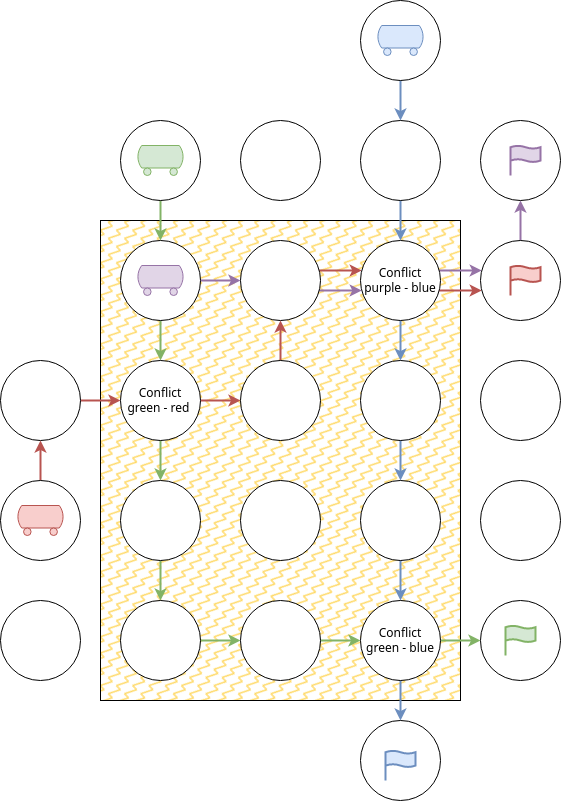
\includegraphics[width=8cm]{img/conflict_window.drawio.png}
\end{figure}


\subsubsection{Diversity}\label{sec:diversity}

Computing diverse path is mainly done using two different diversity measure; based on the Jaccard similarity coefficient (see \cite{habochal21a}), or on the the symmetry difference (also called Hamming distance) (see \cite{hanaka2022computing}) of two sets, we will respectively refer to them as \(diversity_j(\gamma)\) and \(diversity_{\bigtriangleup}(\gamma)\). Both compute diversity among two sets. The Jaccard similarity is defined as the size of the intersection of two sets divided by the size of the union of the two sets. In other words, it is a measure of how similar two sets are, based on the number of elements they have in common. we use them for computing diversity among two set of vertex issued from paths. The Hamming distance is a measure of the difference between two sequences of equal length. It is defined as the number of positions at which the corresponding symbols are different. The difference between the is that the Jaccard index focuses on the number of nodes that two paths have in common, while the Hamming distance focuses on the number of differences between the two paths. If we adapt the notation from the papers, we have
\[
  diversity_j(\gamma)=\sum_{\forall \pi,\pi' \in \gamma}{JaccardCoefficient(vertex(\pi),vertex(\pi'))}
\]

\[
  diversity_{\bigtriangleup}(\gamma)=\sum_{\forall \pi,\pi' \in \gamma}{SymmetryDifference(vertex(\pi),vertex(\pi'))}
\]  





\subsubsection{Distant}\label{sec:distant}
Let \(\gamma\) being a set of path of length \(n\), where all of the path have the same initial and ending position. Let \(\pi,\pi' \in \gamma\) two different paths. \(\pi\) and \(\pi'\) are considered ``most distant'' if no other path in \(\gamma\) have a higher distance. Distance between two paths is computed as such :


\[
  distance(\pi,\pi') = \sum_{k=0}^{n}{dist(\pi(k),\pi'(k))}   
 \] An intermediary function \(dist(V,V) \rightarrow \mathbb{N}\) is necessary; it represents an arbitrary distance function between two vertices, it can be the euclidean distance, length of the shortest path between them\ldots From \(distance\) definition, we can then define the distance from a path to a set of path \(\gamma\): \[
  Distance(\pi,\gamma) = \sum^{\pi'\in\gamma}{distance(\pi,\pi')}   
\] Considering then a set of \(k\) distant paths \(DP \subset \gamma \), \(\pi = pick(\gamma)\), \(\pi \notin DP \), \(\pi\) is distant towards \(DP\) (which means that if we add \(\pi\) to \(DP\), \(DP\) is still distant) if no \(\pi' = pick(\gamma), \pi' \neq \pi\) exist such as \( Distance(\pi,DP) < Distance(\pi',DP)\).


\subsubsection{Heatmap}\label{sec:heatmap}

Heatmap~\cite{atstfestko20a} is about projecting likelihood of presence of agents on vertices. Likelihood refers to the chance of an agent to be positioned at a specific vertex of the graph at a time step \(t\). We introduce the function \(\phi\) which compute likelihood of the vertex \(v\) at time step \(t\) for the set of path \(\gamma\) as such:

\[
  \phi(v, t, \gamma) = \frac{ |\{ \pi | \pi \in \gamma, \pi(t) = v \}|}{|\gamma| }
\]
  
From this definition, we can compute the first three step of an agent with an associated \(|\gamma|=3\) below (figure~\ref{img:heatmap}).

\begin{figure}[H]
  \centering
  \caption{Heatmap example of the first three time step for a \(|\gamma|=3\) }\label{img:heatmap}
  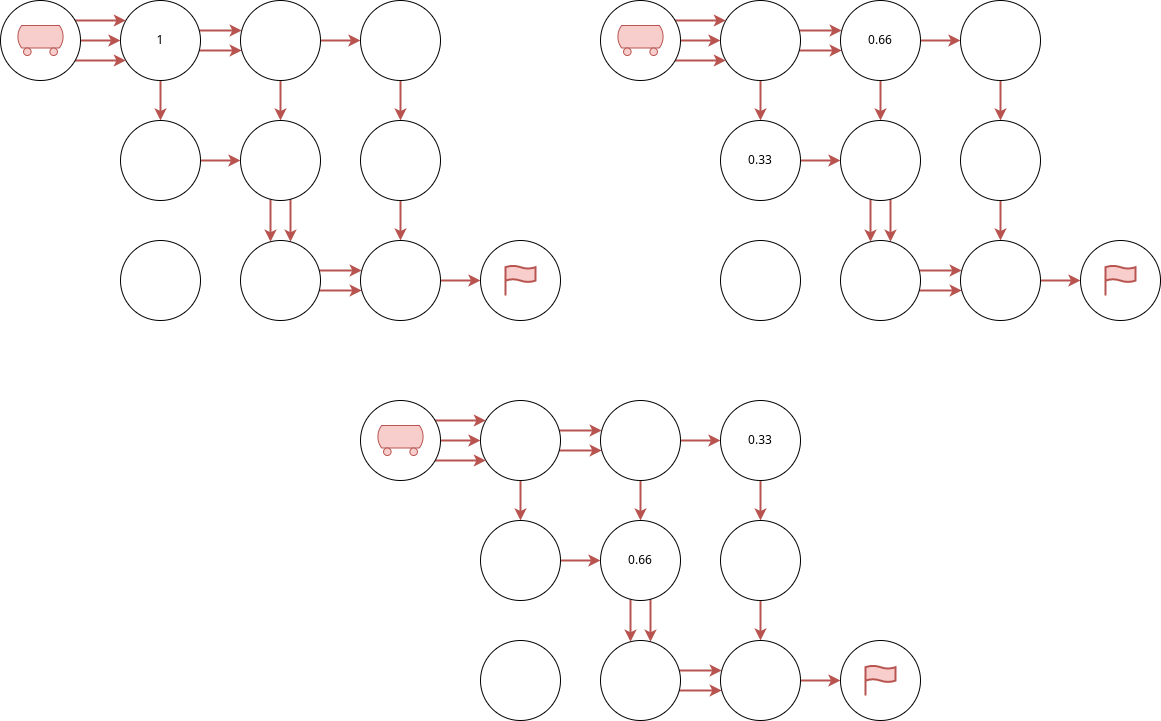
\includegraphics[width=10cm]{img/heatmap.drawio.png}
\end{figure}

This heatmap-per-agent can be used to compute a ``global one'', to do so, for each vertex and for each time step, we sum each \(\phi\) and then divide it by the number of agent (see appendix~\ref{apx:heatmap_and_global}), we will refer to this as \(\Phi\);

\[
  \Phi(v,t,\tau) = \frac{ {\sum^{\gamma \in \tau} }{\phi(v,t,\gamma)}}  {|\tau|}
\]

Computed this way, global heatmaps no longer represent likelihood of presence, rather more an indicator. Both heatmaps together can be useful for different parts of plan merging resolution.

The heatmap we proposed is from the perspective of agents, but it can also be considered from \(\gamma\) scope, especially paths. It can then become a property of a path. These likelihoods per paths gives us information one the path itself; having highs values represent that a vertex is used in different paths of \(\gamma\), a low average value represent a higher diversity, and so on.

It becomes more interesting when we use these values as an objective function; allowing a maximum value for any \(\phi\) in an \(\gamma\) directly influence the way \(\gamma\) would be constituted. For instance, limiting \(\phi\) values of \(\gamma\) for any vertex at maximum of 0.4, forces the number of paths of at least three. Generally, the maximum, minimum and average value of \(\phi\) for any \(\gamma\) gives us information on how the paths are interacting. 



% \subsection{Building interesting \(\tau\)}
% We defined different function that can represent properties of path in \(\tau\), however we can try to imagine set of path of different properties that makes \(\tau\) a ``better'' input for the merging section than a set of path containing a single property. We will start by trying to create interesting \(\gamma\), we will then discuss of the construction of \(\tau\).

% \(\gamma\) represent a set of path for a single agent, figure~\ref{img:building_gamma}~\cite{husvobbass22a,husvobbass22b} represent an instance where, if the blue path is the only one for the agent in \(\gamma\), finding a solution given orange and green path will require additional steps for the merging section, the idea of building an interesting \(\gamma\) is to provide at least both black and blue path. 

% \begin{figure}[H]
%   \centering
%   \caption{Example of providing two shortest path to provide solution}\label{img:building_gamma}
%   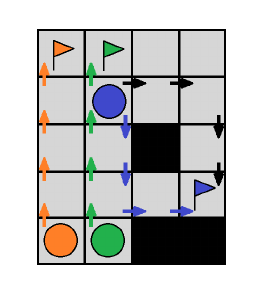
\includegraphics[width=\widthimg]{img/building_gamma.png}
% \end{figure}

% In the example~\ref{img:building_gamma} above, providing all the shortest path is ``easy'' (in terms of space search) how ever, on bigger instances, the number of possible shortest path is raising exponentially. Three approach can be used to build \(\gamma\).
% On the first hand, we can then imagine pre-defined \(\gamma\) requirements; as shown in figure~\ref{img:building_gamma}, black and blue path are two distant shortest path, furthermore, a set of three distant shortest path seems to be an interesting combination (see~\nameref{img:three_distant_path}, see~\cite{husvobbass22a,husvobbass22b}); the coverage of the graph (see~\nameref{sec:graph_coverage}) related to the number of path provided is quite interesting in low-obstacles density instances case, plus, by definition, the number of overlapping is guarantee to be the lowest given the number of distant paths.

% \begin{figure}[H]
%   \centering
%   \caption{Three distant path}\label{img:three_distant_path}
%   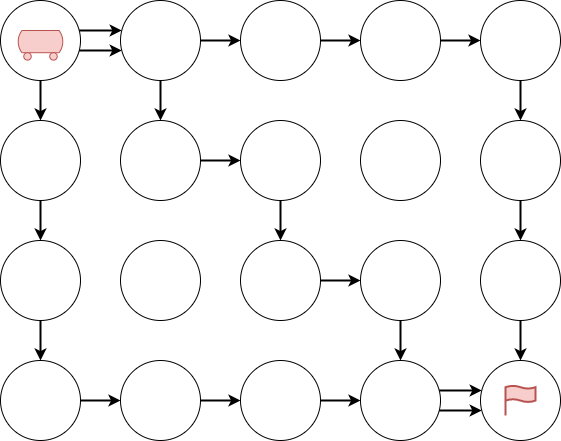
\includegraphics[width=\widthimg]{img/three_distant_path.drawio.png}
% \end{figure}

% Distant paths are part of the strategies provided in paper~\cite{husvobbass22a,husvobbass22b}, they also describe \textbf{Single path}, \textbf{All paths} which correspond to all the shortest path possible for an agent, \textbf{Random paths} which correspond to a subset of the previous strategy, furthermore the size of the subset is at most of size \(\frac{|SP|}{|SP^i|}\). The benchmark associated to the paper shows that the the Single Path strategy comes with the best result on both optimal and suboptimal strategies.

% On the other hand, we can automate \(gamma\) requirements through benchmarks and grid tuning; given a set of different cost function, we can determine which combination gives the best result by running tests on instances; number of instance solved, computation time, optimality...